\documentclass[1p]{elsarticle_modified}
%\bibliographystyle{elsarticle-num}

%\usepackage[colorlinks]{hyperref}
%\usepackage{abbrmath_seonhwa} %\Abb, \Ascr, \Acal ,\Abf, \Afrak
\usepackage{amsfonts}
\usepackage{amssymb}
\usepackage{amsmath}
\usepackage{amsthm}
\usepackage{scalefnt}
\usepackage{amsbsy}
\usepackage{kotex}
\usepackage{caption}
\usepackage{subfig}
\usepackage{color}
\usepackage{graphicx}
\usepackage{xcolor} %% white, black, red, green, blue, cyan, magenta, yellow
\usepackage{float}
\usepackage{setspace}
\usepackage{hyperref}

\usepackage{tikz}
\usetikzlibrary{arrows}

\usepackage{multirow}
\usepackage{array} % fixed length table
\usepackage{hhline}

%%%%%%%%%%%%%%%%%%%%%
\makeatletter
\renewcommand*\env@matrix[1][\arraystretch]{%
	\edef\arraystretch{#1}%
	\hskip -\arraycolsep
	\let\@ifnextchar\new@ifnextchar
	\array{*\c@MaxMatrixCols c}}
\makeatother %https://tex.stackexchange.com/questions/14071/how-can-i-increase-the-line-spacing-in-a-matrix
%%%%%%%%%%%%%%%

\usepackage[normalem]{ulem}

\newcommand{\msout}[1]{\ifmmode\text{\sout{\ensuremath{#1}}}\else\sout{#1}\fi}
%SOURCE: \msout is \stkout macro in https://tex.stackexchange.com/questions/20609/strikeout-in-math-mode

\newcommand{\cancel}[1]{
	\ifmmode
	{\color{red}\msout{#1}}
	\else
	{\color{red}\sout{#1}}
	\fi
}

\newcommand{\add}[1]{
	{\color{blue}\uwave{#1}}
}

\newcommand{\replace}[2]{
	\ifmmode
	{\color{red}\msout{#1}}{\color{blue}\uwave{#2}}
	\else
	{\color{red}\sout{#1}}{\color{blue}\uwave{#2}}
	\fi
}

\newcommand{\Sol}{\mathcal{S}} %segment
\newcommand{\D}{D} %diagram
\newcommand{\A}{\mathcal{A}} %arc


%%%%%%%%%%%%%%%%%%%%%%%%%%%%%5 test

\def\sl{\operatorname{\textup{SL}}(2,\Cbb)}
\def\psl{\operatorname{\textup{PSL}}(2,\Cbb)}
\def\quan{\mkern 1mu \triangleright \mkern 1mu}

\theoremstyle{definition}
\newtheorem{thm}{Theorem}[section]
\newtheorem{prop}[thm]{Proposition}
\newtheorem{lem}[thm]{Lemma}
\newtheorem{ques}[thm]{Question}
\newtheorem{cor}[thm]{Corollary}
\newtheorem{defn}[thm]{Definition}
\newtheorem{exam}[thm]{Example}
\newtheorem{rmk}[thm]{Remark}
\newtheorem{alg}[thm]{Algorithm}

\newcommand{\I}{\sqrt{-1}}
\begin{document}

%\begin{frontmatter}
%
%\title{Boundary parabolic representations of knots up to 8 crossings}
%
%%% Group authors per affiliation:
%\author{Yunhi Cho} 
%\address{Department of Mathematics, University of Seoul, Seoul, Korea}
%\ead{yhcho@uos.ac.kr}
%
%
%\author{Seonhwa Kim} %\fnref{s_kim}}
%\address{Center for Geometry and Physics, Institute for Basic Science, Pohang, 37673, Korea}
%\ead{ryeona17@ibs.re.kr}
%
%\author{Hyuk Kim}
%\address{Department of Mathematical Sciences, Seoul National University, Seoul 08826, Korea}
%\ead{hyukkim@snu.ac.kr}
%
%\author{Seokbeom Yoon}
%\address{Department of Mathematical Sciences, Seoul National University, Seoul, 08826,  Korea}
%\ead{sbyoon15@snu.ac.kr}
%
%\begin{abstract}
%We find all boundary parabolic representation of knots up to 8 crossings.
%
%\end{abstract}
%\begin{keyword}
%    \MSC[2010] 57M25 
%\end{keyword}
%
%\end{frontmatter}

%\linenumbers
%\tableofcontents
%
\newcommand\colored[1]{\textcolor{white}{\rule[-0.35ex]{0.8em}{1.4ex}}\kern-0.8em\color{red} #1}%
%\newcommand\colored[1]{\textcolor{white}{ #1}\kern-2.17ex	\textcolor{white}{ #1}\kern-1.81ex	\textcolor{white}{ #1}\kern-2.15ex\color{red}#1	}

{\Large $\underline{12a_{0382}~(K12a_{0382})}$}

\setlength{\tabcolsep}{10pt}
\renewcommand{\arraystretch}{1.6}
\vspace{1cm}\begin{tabular}{m{100pt}>{\centering\arraybackslash}m{274pt}}
\multirow{5}{120pt}{
	\centering
	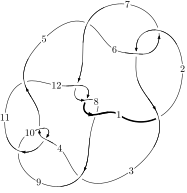
\includegraphics[width=112pt]{../../../GIT/diagram.site/Diagrams/png/1183_12a_0382.png}\\
\ \ \ A knot diagram\footnotemark}&
\allowdisplaybreaks
\textbf{Linearized knot diagam} \\
\cline{2-2}
 &
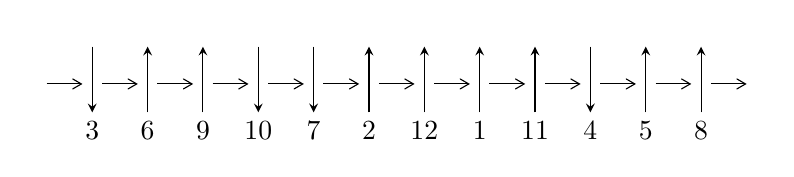
\begin{tikzpicture}[x=20pt, y=17pt]
	% nodes
	\node (C0) at (0, 0) {};
	\node (C1) at (1, 0) {};
	\node (C1U) at (1, +1) {};
	\node (C1D) at (1, -1) {3};

	\node (C2) at (2, 0) {};
	\node (C2U) at (2, +1) {};
	\node (C2D) at (2, -1) {6};

	\node (C3) at (3, 0) {};
	\node (C3U) at (3, +1) {};
	\node (C3D) at (3, -1) {9};

	\node (C4) at (4, 0) {};
	\node (C4U) at (4, +1) {};
	\node (C4D) at (4, -1) {10};

	\node (C5) at (5, 0) {};
	\node (C5U) at (5, +1) {};
	\node (C5D) at (5, -1) {7};

	\node (C6) at (6, 0) {};
	\node (C6U) at (6, +1) {};
	\node (C6D) at (6, -1) {2};

	\node (C7) at (7, 0) {};
	\node (C7U) at (7, +1) {};
	\node (C7D) at (7, -1) {12};

	\node (C8) at (8, 0) {};
	\node (C8U) at (8, +1) {};
	\node (C8D) at (8, -1) {1};

	\node (C9) at (9, 0) {};
	\node (C9U) at (9, +1) {};
	\node (C9D) at (9, -1) {11};

	\node (C10) at (10, 0) {};
	\node (C10U) at (10, +1) {};
	\node (C10D) at (10, -1) {4};

	\node (C11) at (11, 0) {};
	\node (C11U) at (11, +1) {};
	\node (C11D) at (11, -1) {5};

	\node (C12) at (12, 0) {};
	\node (C12U) at (12, +1) {};
	\node (C12D) at (12, -1) {8};
	\node (C13) at (13, 0) {};

	% arrows
	\draw[->,>={angle 60}]
	(C0) edge (C1) (C1) edge (C2) (C2) edge (C3) (C3) edge (C4) (C4) edge (C5) (C5) edge (C6) (C6) edge (C7) (C7) edge (C8) (C8) edge (C9) (C9) edge (C10) (C10) edge (C11) (C11) edge (C12) (C12) edge (C13) ;	\draw[->,>=stealth]
	(C1U) edge (C1D) (C2D) edge (C2U) (C3D) edge (C3U) (C4U) edge (C4D) (C5U) edge (C5D) (C6D) edge (C6U) (C7D) edge (C7U) (C8D) edge (C8U) (C9D) edge (C9U) (C10U) edge (C10D) (C11D) edge (C11U) (C12D) edge (C12U) ;
	\end{tikzpicture} \\
\hhline{~~} \\& 
\textbf{Solving Sequence} \\ \cline{2-2} 
 &
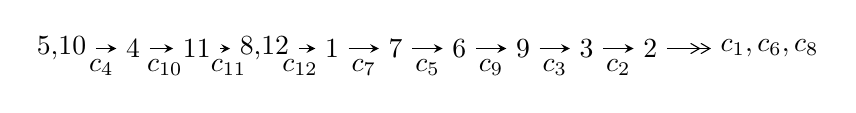
\begin{tikzpicture}[x=23pt, y=7pt]
	% node
	\node (A0) at (-1/8, 0) {5,10};
	\node (A1) at (1, 0) {4};
	\node (A2) at (2, 0) {11};
	\node (A3) at (49/16, 0) {8,12};
	\node (A4) at (33/8, 0) {1};
	\node (A5) at (41/8, 0) {7};
	\node (A6) at (49/8, 0) {6};
	\node (A7) at (57/8, 0) {9};
	\node (A8) at (65/8, 0) {3};
	\node (A9) at (73/8, 0) {2};
	\node (C1) at (1/2, -1) {$c_{4}$};
	\node (C2) at (3/2, -1) {$c_{10}$};
	\node (C3) at (5/2, -1) {$c_{11}$};
	\node (C4) at (29/8, -1) {$c_{12}$};
	\node (C5) at (37/8, -1) {$c_{7}$};
	\node (C6) at (45/8, -1) {$c_{5}$};
	\node (C7) at (53/8, -1) {$c_{9}$};
	\node (C8) at (61/8, -1) {$c_{3}$};
	\node (C9) at (69/8, -1) {$c_{2}$};
	\node (A10) at (11, 0) {$c_{1},c_{6},c_{8}$};

	% edge
	\draw[->,>=stealth]	
	(A0) edge (A1) (A1) edge (A2) (A2) edge (A3) (A3) edge (A4) (A4) edge (A5) (A5) edge (A6) (A6) edge (A7) (A7) edge (A8) (A8) edge (A9) ;
	\draw[->>,>={angle 60}]	
	(A9) edge (A10);
\end{tikzpicture} \\ 

\end{tabular} \\

\footnotetext{
The image of knot diagram is generated by the software ``\textbf{Draw programme}" developed by Andrew Bartholomew(\url{http://www.layer8.co.uk/maths/draw/index.htm\#Running-draw}), where we modified some parts for our purpose(\url{https://github.com/CATsTAILs/LinksPainter}).
}\phantom \\ \newline 
\centering \textbf{Ideals for irreducible components\footnotemark of $X_{\text{par}}$} 
 
\begin{align*}
I^u_{1}&=\langle 
5.25760\times10^{40} u^{79}-7.60567\times10^{40} u^{78}+\cdots+2.32478\times10^{40} b+1.39471\times10^{38},\\
\phantom{I^u_{1}}&\phantom{= \langle  }2.10242\times10^{40} u^{79}-1.11824\times10^{40} u^{78}+\cdots+2.32478\times10^{40} a-6.38186\times10^{40},\;u^{80}- u^{79}+\cdots+4 u-4\rangle \\
I^u_{2}&=\langle 
u^2 a+u^3+2 b+u,\;2 u^3 a-2 u^2 a+2 a^2+5 u^2-4 a+2 u+6,\;u^4+2 u^2+2\rangle \\
\\
I^v_{1}&=\langle 
a,\;b+v-1,\;v^2- v+1\rangle \\
\end{align*}
\raggedright * 3 irreducible components of $\dim_{\mathbb{C}}=0$, with total 90 representations.\\
\footnotetext{All coefficients of polynomials are rational numbers. But the coefficients are sometimes approximated in decimal forms when there is not enough margin.}
\newpage
\renewcommand{\arraystretch}{1}
\centering \section*{I. $I^u_{1}= \langle 5.26\times10^{40} u^{79}-7.61\times10^{40} u^{78}+\cdots+2.32\times10^{40} b+1.39\times10^{38},\;2.10\times10^{40} u^{79}-1.12\times10^{40} u^{78}+\cdots+2.32\times10^{40} a-6.38\times10^{40},\;u^{80}- u^{79}+\cdots+4 u-4 \rangle$}
\flushleft \textbf{(i) Arc colorings}\\
\begin{tabular}{m{7pt} m{180pt} m{7pt} m{180pt} }
\flushright $a_{5}=$&$\begin{pmatrix}1\\0\end{pmatrix}$ \\
\flushright $a_{10}=$&$\begin{pmatrix}0\\u\end{pmatrix}$ \\
\flushright $a_{4}=$&$\begin{pmatrix}1\\- u^2\end{pmatrix}$ \\
\flushright $a_{11}=$&$\begin{pmatrix}- u\\u^3+u\end{pmatrix}$ \\
\flushright $a_{8}=$&$\begin{pmatrix}-0.904354 u^{79}+0.481007 u^{78}+\cdots-1.07187 u+2.74514\\-2.26155 u^{79}+3.27156 u^{78}+\cdots+11.4214 u-0.00599931\end{pmatrix}$ \\
\flushright $a_{12}=$&$\begin{pmatrix}u^3\\u^3+u\end{pmatrix}$ \\
\flushright $a_{1}=$&$\begin{pmatrix}0.904354 u^{79}-0.481007 u^{78}+\cdots+1.07187 u-2.74514\\-1.40429 u^{79}+2.20008 u^{78}+\cdots+9.49738 u-1.69939\end{pmatrix}$ \\
\flushright $a_{7}=$&$\begin{pmatrix}-1.13657 u^{79}+1.84293 u^{78}+\cdots+7.02460 u-2.17652\\-1.70006 u^{79}+2.60937 u^{78}+\cdots+9.55138 u-0.627990\end{pmatrix}$ \\
\flushright $a_{6}=$&$\begin{pmatrix}-0.0263781 u^{79}+1.69363 u^{78}+\cdots+11.1328 u-6.06948\\1.38845 u^{79}-2.43528 u^{78}+\cdots-9.84146 u+1.92979\end{pmatrix}$ \\
\flushright $a_{9}=$&$\begin{pmatrix}- u^3\\u^5+u^3+u\end{pmatrix}$ \\
\flushright $a_{3}=$&$\begin{pmatrix}- u^6- u^4+1\\u^8+2 u^6+2 u^4\end{pmatrix}$ \\
\flushright $a_{2}=$&$\begin{pmatrix}2.09245 u^{79}-2.33106 u^{78}+\cdots-5.71599 u-2.00297\\-0.784122 u^{79}+0.549512 u^{78}+\cdots+0.603346 u+2.47675\end{pmatrix}$\\&\end{tabular}
\flushleft \textbf{(ii) Obstruction class $= -1$}\\~\\
\flushleft \textbf{(iii) Cusp Shapes $= 5.47878 u^{79}-9.68885 u^{78}+\cdots-54.6240 u+21.2301$}\\~\\
\newpage\renewcommand{\arraystretch}{1}
\flushleft \textbf{(iv) u-Polynomials at the component}\newline \\
\begin{tabular}{m{50pt}|m{274pt}}
Crossings & \hspace{64pt}u-Polynomials at each crossing \\
\hline $$\begin{aligned}c_{1},c_{5}\end{aligned}$$&$\begin{aligned}
&u^{80}+24 u^{79}+\cdots+8 u+1
\end{aligned}$\\
\hline $$\begin{aligned}c_{2},c_{6}\end{aligned}$$&$\begin{aligned}
&u^{80}-2 u^{79}+\cdots-2 u+1
\end{aligned}$\\
\hline $$\begin{aligned}c_{3},c_{11}\end{aligned}$$&$\begin{aligned}
&u^{80}+u^{79}+\cdots-452 u-404
\end{aligned}$\\
\hline $$\begin{aligned}c_{4},c_{10}\end{aligned}$$&$\begin{aligned}
&u^{80}- u^{79}+\cdots+4 u-4
\end{aligned}$\\
\hline $$\begin{aligned}c_{7},c_{8},c_{12}\end{aligned}$$&$\begin{aligned}
&u^{80}-3 u^{79}+\cdots-83 u-13
\end{aligned}$\\
\hline $$\begin{aligned}c_{9}\end{aligned}$$&$\begin{aligned}
&u^{80}-45 u^{79}+\cdots-80 u+16
\end{aligned}$\\
\hline
\end{tabular}\\~\\
\newpage\renewcommand{\arraystretch}{1}
\flushleft \textbf{(v) Riley Polynomials at the component}\newline \\
\begin{tabular}{m{50pt}|m{274pt}}
Crossings & \hspace{64pt}Riley Polynomials at each crossing \\
\hline $$\begin{aligned}c_{1},c_{5}\end{aligned}$$&$\begin{aligned}
&y^{80}+72 y^{79}+\cdots-56 y+1
\end{aligned}$\\
\hline $$\begin{aligned}c_{2},c_{6}\end{aligned}$$&$\begin{aligned}
&y^{80}+24 y^{79}+\cdots+8 y+1
\end{aligned}$\\
\hline $$\begin{aligned}c_{3},c_{11}\end{aligned}$$&$\begin{aligned}
&y^{80}-75 y^{79}+\cdots-2017456 y+163216
\end{aligned}$\\
\hline $$\begin{aligned}c_{4},c_{10}\end{aligned}$$&$\begin{aligned}
&y^{80}+45 y^{79}+\cdots+80 y+16
\end{aligned}$\\
\hline $$\begin{aligned}c_{7},c_{8},c_{12}\end{aligned}$$&$\begin{aligned}
&y^{80}-85 y^{79}+\cdots-3353 y+169
\end{aligned}$\\
\hline $$\begin{aligned}c_{9}\end{aligned}$$&$\begin{aligned}
&y^{80}-15 y^{79}+\cdots-1792 y+256
\end{aligned}$\\
\hline
\end{tabular}\\~\\
\newpage\flushleft \textbf{(vi) Complex Volumes and Cusp Shapes}
$$\begin{array}{c|c|c}  
\text{Solutions to }I^u_{1}& \I (\text{vol} + \sqrt{-1}CS) & \text{Cusp shape}\\
 \hline 
\begin{aligned}
u &= -0.465995 + 0.890027 I \\
a &= -0.441303 + 0.096283 I \\
b &= -1.45500 - 0.66755 I\end{aligned}
 & \phantom{-}1.05476 + 4.92101 I & \phantom{-0.000000 } 0 \\ \hline\begin{aligned}
u &= -0.465995 - 0.890027 I \\
a &= -0.441303 - 0.096283 I \\
b &= -1.45500 + 0.66755 I\end{aligned}
 & \phantom{-}1.05476 - 4.92101 I & \phantom{-0.000000 } 0 \\ \hline\begin{aligned}
u &= \phantom{-}0.138898 + 0.959842 I \\
a &= -1.40999 + 1.38132 I \\
b &= -0.376133 + 1.039330 I\end{aligned}
 & \phantom{-}3.54764 + 1.95603 I & \phantom{-}12.28857 - 3.06785 I \\ \hline\begin{aligned}
u &= \phantom{-}0.138898 - 0.959842 I \\
a &= -1.40999 - 1.38132 I \\
b &= -0.376133 - 1.039330 I\end{aligned}
 & \phantom{-}3.54764 - 1.95603 I & \phantom{-}12.28857 + 3.06785 I \\ \hline\begin{aligned}
u &= -0.255592 + 0.927697 I \\
a &= \phantom{-}1.34947 + 2.03332 I \\
b &= \phantom{-}0.009870 + 1.328880 I\end{aligned}
 & \phantom{-}3.00368 + 3.13036 I & \phantom{-}10.09819 - 3.88096 I \\ \hline\begin{aligned}
u &= -0.255592 - 0.927697 I \\
a &= \phantom{-}1.34947 - 2.03332 I \\
b &= \phantom{-}0.009870 - 1.328880 I\end{aligned}
 & \phantom{-}3.00368 - 3.13036 I & \phantom{-}10.09819 + 3.88096 I \\ \hline\begin{aligned}
u &= -0.407948 + 0.961740 I \\
a &= -1.228550 - 0.288226 I \\
b &= -0.209191 - 0.418092 I\end{aligned}
 & \phantom{-}1.82577 + 1.64059 I & \phantom{-0.000000 } 0 \\ \hline\begin{aligned}
u &= -0.407948 - 0.961740 I \\
a &= -1.228550 + 0.288226 I \\
b &= -0.209191 + 0.418092 I\end{aligned}
 & \phantom{-}1.82577 - 1.64059 I & \phantom{-0.000000 } 0 \\ \hline\begin{aligned}
u &= \phantom{-}0.482819 + 0.934965 I \\
a &= \phantom{-}1.079240 - 0.701792 I \\
b &= -0.200382 - 0.585726 I\end{aligned}
 & \phantom{-}1.16955 - 6.69579 I & \phantom{-0.000000 } 0 \\ \hline\begin{aligned}
u &= \phantom{-}0.482819 - 0.934965 I \\
a &= \phantom{-}1.079240 + 0.701792 I \\
b &= -0.200382 + 0.585726 I\end{aligned}
 & \phantom{-}1.16955 + 6.69579 I & \phantom{-0.000000 } 0\\
 \hline 
 \end{array}$$\newpage$$\begin{array}{c|c|c}  
\text{Solutions to }I^u_{1}& \I (\text{vol} + \sqrt{-1}CS) & \text{Cusp shape}\\
 \hline 
\begin{aligned}
u &= \phantom{-}0.304527 + 1.033480 I \\
a &= \phantom{-}0.389055 + 0.408709 I \\
b &= \phantom{-}0.914489 - 0.830590 I\end{aligned}
 & \phantom{-}4.63163 - 3.09536 I & \phantom{-0.000000 } 0 \\ \hline\begin{aligned}
u &= \phantom{-}0.304527 - 1.033480 I \\
a &= \phantom{-}0.389055 - 0.408709 I \\
b &= \phantom{-}0.914489 + 0.830590 I\end{aligned}
 & \phantom{-}4.63163 + 3.09536 I & \phantom{-0.000000 } 0 \\ \hline\begin{aligned}
u &= -0.718292 + 0.564408 I \\
a &= \phantom{-}0.30054 + 1.50770 I \\
b &= -0.699048 + 0.453179 I\end{aligned}
 & \phantom{-}6.00409 - 4.34016 I & \phantom{-}7.41183 + 2.66481 I \\ \hline\begin{aligned}
u &= -0.718292 - 0.564408 I \\
a &= \phantom{-}0.30054 - 1.50770 I \\
b &= -0.699048 - 0.453179 I\end{aligned}
 & \phantom{-}6.00409 + 4.34016 I & \phantom{-}7.41183 - 2.66481 I \\ \hline\begin{aligned}
u &= -0.222929 + 0.884136 I \\
a &= -0.215941 + 0.267184 I \\
b &= -1.07893 - 1.42958 I\end{aligned}
 & \phantom{-}2.79044 - 1.07850 I & \phantom{-}9.91240 - 0.16778 I \\ \hline\begin{aligned}
u &= -0.222929 - 0.884136 I \\
a &= -0.215941 - 0.267184 I \\
b &= -1.07893 + 1.42958 I\end{aligned}
 & \phantom{-}2.79044 + 1.07850 I & \phantom{-}9.91240 + 0.16778 I \\ \hline\begin{aligned}
u &= -0.897293 + 0.111616 I \\
a &= \phantom{-}0.271629 - 0.075634 I \\
b &= \phantom{-}2.77247 + 0.37666 I\end{aligned}
 & \phantom{-}13.07070 - 4.01680 I & \phantom{-}9.61331 + 0.81202 I \\ \hline\begin{aligned}
u &= -0.897293 - 0.111616 I \\
a &= \phantom{-}0.271629 + 0.075634 I \\
b &= \phantom{-}2.77247 - 0.37666 I\end{aligned}
 & \phantom{-}13.07070 + 4.01680 I & \phantom{-}9.61331 - 0.81202 I \\ \hline\begin{aligned}
u &= \phantom{-}0.890645 + 0.137467 I \\
a &= -0.265905 - 0.093191 I \\
b &= -2.73738 + 0.46410 I\end{aligned}
 & \phantom{-}12.1328 + 10.4310 I & \phantom{-}8.31438 - 5.43420 I \\ \hline\begin{aligned}
u &= \phantom{-}0.890645 - 0.137467 I \\
a &= -0.265905 + 0.093191 I \\
b &= -2.73738 - 0.46410 I\end{aligned}
 & \phantom{-}12.1328 - 10.4310 I & \phantom{-}8.31438 + 5.43420 I\\
 \hline 
 \end{array}$$\newpage$$\begin{array}{c|c|c}  
\text{Solutions to }I^u_{1}& \I (\text{vol} + \sqrt{-1}CS) & \text{Cusp shape}\\
 \hline 
\begin{aligned}
u &= \phantom{-}0.473965 + 0.759787 I \\
a &= \phantom{-}0.499997 - 0.399523 I \\
b &= -0.386214 + 0.092533 I\end{aligned}
 & -2.89498 - 1.99126 I & -3.21441 + 4.67828 I \\ \hline\begin{aligned}
u &= \phantom{-}0.473965 - 0.759787 I \\
a &= \phantom{-}0.499997 + 0.399523 I \\
b &= -0.386214 - 0.092533 I\end{aligned}
 & -2.89498 + 1.99126 I & -3.21441 - 4.67828 I \\ \hline\begin{aligned}
u &= \phantom{-}0.730077 + 0.516813 I \\
a &= -0.33209 + 1.43938 I \\
b &= \phantom{-}0.692107 + 0.425189 I\end{aligned}
 & \phantom{-}6.24399 - 1.64013 I & \phantom{-}7.94611 + 2.56376 I \\ \hline\begin{aligned}
u &= \phantom{-}0.730077 - 0.516813 I \\
a &= -0.33209 - 1.43938 I \\
b &= \phantom{-}0.692107 - 0.425189 I\end{aligned}
 & \phantom{-}6.24399 + 1.64013 I & \phantom{-}7.94611 - 2.56376 I \\ \hline\begin{aligned}
u &= -0.621172 + 0.959007 I \\
a &= -0.596898 - 0.048619 I \\
b &= -1.37777 - 0.41758 I\end{aligned}
 & \phantom{-}7.15122 + 9.41978 I & \phantom{-0.000000 } 0 \\ \hline\begin{aligned}
u &= -0.621172 - 0.959007 I \\
a &= -0.596898 + 0.048619 I \\
b &= -1.37777 + 0.41758 I\end{aligned}
 & \phantom{-}7.15122 - 9.41978 I & \phantom{-0.000000 } 0 \\ \hline\begin{aligned}
u &= -0.853744\phantom{ +0.000000I} \\
a &= \phantom{-}0.244881\phantom{ +0.000000I} \\
b &= \phantom{-}3.05747\phantom{ +0.000000I}\end{aligned}
 & \phantom{-}8.46558\phantom{ +0.000000I} & \phantom{-}10.3700\phantom{ +0.000000I} \\ \hline\begin{aligned}
u &= -0.835740 + 0.069667 I \\
a &= \phantom{-}0.121736 - 0.573005 I \\
b &= -0.860834 - 0.096641 I\end{aligned}
 & \phantom{-}5.16321 - 5.92875 I & \phantom{-}6.57093 + 5.18628 I \\ \hline\begin{aligned}
u &= -0.835740 - 0.069667 I \\
a &= \phantom{-}0.121736 + 0.573005 I \\
b &= -0.860834 + 0.096641 I\end{aligned}
 & \phantom{-}5.16321 + 5.92875 I & \phantom{-}6.57093 - 5.18628 I \\ \hline\begin{aligned}
u &= \phantom{-}0.608825 + 0.993182 I \\
a &= \phantom{-}0.636243 - 0.025508 I \\
b &= \phantom{-}1.345400 - 0.421772 I\end{aligned}
 & \phantom{-}7.63224 - 3.42695 I & \phantom{-0.000000 } 0\\
 \hline 
 \end{array}$$\newpage$$\begin{array}{c|c|c}  
\text{Solutions to }I^u_{1}& \I (\text{vol} + \sqrt{-1}CS) & \text{Cusp shape}\\
 \hline 
\begin{aligned}
u &= \phantom{-}0.608825 - 0.993182 I \\
a &= \phantom{-}0.636243 + 0.025508 I \\
b &= \phantom{-}1.345400 + 0.421772 I\end{aligned}
 & \phantom{-}7.63224 + 3.42695 I & \phantom{-0.000000 } 0 \\ \hline\begin{aligned}
u &= \phantom{-}0.830514 + 0.028983 I \\
a &= -0.168471 - 0.606307 I \\
b &= \phantom{-}0.834469 - 0.116020 I\end{aligned}
 & \phantom{-}5.51190 - 0.08562 I & \phantom{-}7.53170 - 0.02621 I \\ \hline\begin{aligned}
u &= \phantom{-}0.830514 - 0.028983 I \\
a &= -0.168471 + 0.606307 I \\
b &= \phantom{-}0.834469 + 0.116020 I\end{aligned}
 & \phantom{-}5.51190 + 0.08562 I & \phantom{-}7.53170 + 0.02621 I \\ \hline\begin{aligned}
u &= \phantom{-}0.814288 + 0.058409 I \\
a &= -0.218467 - 0.037164 I \\
b &= -3.20383 + 0.31940 I\end{aligned}
 & \phantom{-}4.47676 + 4.08811 I & \phantom{-}5.94358 - 3.55557 I \\ \hline\begin{aligned}
u &= \phantom{-}0.814288 - 0.058409 I \\
a &= -0.218467 + 0.037164 I \\
b &= -3.20383 - 0.31940 I\end{aligned}
 & \phantom{-}4.47676 - 4.08811 I & \phantom{-}5.94358 + 3.55557 I \\ \hline\begin{aligned}
u &= -0.420036 + 1.121960 I \\
a &= -1.312780 + 0.338786 I \\
b &= -0.980693 - 0.347373 I\end{aligned}
 & \phantom{-}2.29503 + 1.39582 I & \phantom{-0.000000 } 0 \\ \hline\begin{aligned}
u &= -0.420036 - 1.121960 I \\
a &= -1.312780 - 0.338786 I \\
b &= -0.980693 + 0.347373 I\end{aligned}
 & \phantom{-}2.29503 - 1.39582 I & \phantom{-0.000000 } 0 \\ \hline\begin{aligned}
u &= \phantom{-}0.022114 + 1.201810 I \\
a &= \phantom{-}0.026017 + 0.667704 I \\
b &= \phantom{-}0.051525 - 0.715255 I\end{aligned}
 & \phantom{-}12.02500 - 3.18270 I & \phantom{-0.000000 } 0 \\ \hline\begin{aligned}
u &= \phantom{-}0.022114 - 1.201810 I \\
a &= \phantom{-}0.026017 - 0.667704 I \\
b &= \phantom{-}0.051525 + 0.715255 I\end{aligned}
 & \phantom{-}12.02500 + 3.18270 I & \phantom{-0.000000 } 0 \\ \hline\begin{aligned}
u &= \phantom{-}0.427711 + 1.135650 I \\
a &= \phantom{-}0.800534 + 0.574575 I \\
b &= \phantom{-}0.980152 - 0.405539 I\end{aligned}
 & \phantom{-}4.29603 - 3.85211 I & \phantom{-0.000000 } 0\\
 \hline 
 \end{array}$$\newpage$$\begin{array}{c|c|c}  
\text{Solutions to }I^u_{1}& \I (\text{vol} + \sqrt{-1}CS) & \text{Cusp shape}\\
 \hline 
\begin{aligned}
u &= \phantom{-}0.427711 - 1.135650 I \\
a &= \phantom{-}0.800534 - 0.574575 I \\
b &= \phantom{-}0.980152 + 0.405539 I\end{aligned}
 & \phantom{-}4.29603 + 3.85211 I & \phantom{-0.000000 } 0 \\ \hline\begin{aligned}
u &= -0.462927 + 0.633291 I \\
a &= \phantom{-}0.53377 + 1.87620 I \\
b &= -0.529788 + 0.626997 I\end{aligned}
 & \phantom{-}0.307290 - 0.999281 I & \phantom{-}1.095810 - 0.533831 I \\ \hline\begin{aligned}
u &= -0.462927 - 0.633291 I \\
a &= \phantom{-}0.53377 - 1.87620 I \\
b &= -0.529788 - 0.626997 I\end{aligned}
 & \phantom{-}0.307290 + 0.999281 I & \phantom{-}1.095810 + 0.533831 I \\ \hline\begin{aligned}
u &= \phantom{-}0.484079 + 1.119780 I \\
a &= \phantom{-}0.866749 + 0.224504 I \\
b &= \phantom{-}1.140810 - 0.396001 I\end{aligned}
 & \phantom{-}3.93599 - 3.81750 I & \phantom{-0.000000 } 0 \\ \hline\begin{aligned}
u &= \phantom{-}0.484079 - 1.119780 I \\
a &= \phantom{-}0.866749 - 0.224504 I \\
b &= \phantom{-}1.140810 + 0.396001 I\end{aligned}
 & \phantom{-}3.93599 + 3.81750 I & \phantom{-0.000000 } 0 \\ \hline\begin{aligned}
u &= -0.213622 + 0.748341 I \\
a &= -0.526734 + 0.180517 I \\
b &= -0.072777 + 0.311265 I\end{aligned}
 & \phantom{-}0.469913 + 1.044090 I & \phantom{-}6.86138 - 6.22374 I \\ \hline\begin{aligned}
u &= -0.213622 - 0.748341 I \\
a &= -0.526734 - 0.180517 I \\
b &= -0.072777 - 0.311265 I\end{aligned}
 & \phantom{-}0.469913 - 1.044090 I & \phantom{-}6.86138 + 6.22374 I \\ \hline\begin{aligned}
u &= -0.477124 + 1.149760 I \\
a &= -1.013430 + 0.942548 I \\
b &= -1.032000 - 0.244669 I\end{aligned}
 & \phantom{-}1.86076 + 6.51679 I & \phantom{-0.000000 } 0 \\ \hline\begin{aligned}
u &= -0.477124 - 1.149760 I \\
a &= -1.013430 - 0.942548 I \\
b &= -1.032000 + 0.244669 I\end{aligned}
 & \phantom{-}1.86076 - 6.51679 I & \phantom{-0.000000 } 0 \\ \hline\begin{aligned}
u &= \phantom{-}0.478853 + 0.518342 I \\
a &= \phantom{-}0.157255 - 0.210245 I \\
b &= -0.243674 + 0.798703 I\end{aligned}
 & \phantom{-}0.01114 + 2.66370 I & \phantom{-}0.22333 - 3.59171 I\\
 \hline 
 \end{array}$$\newpage$$\begin{array}{c|c|c}  
\text{Solutions to }I^u_{1}& \I (\text{vol} + \sqrt{-1}CS) & \text{Cusp shape}\\
 \hline 
\begin{aligned}
u &= \phantom{-}0.478853 - 0.518342 I \\
a &= \phantom{-}0.157255 + 0.210245 I \\
b &= -0.243674 - 0.798703 I\end{aligned}
 & \phantom{-}0.01114 - 2.66370 I & \phantom{-}0.22333 + 3.59171 I \\ \hline\begin{aligned}
u &= \phantom{-}0.430621 + 1.222960 I \\
a &= -3.99939 - 1.81832 I \\
b &= -3.41999 + 0.85134 I\end{aligned}
 & \phantom{-}8.27741 - 0.27610 I & \phantom{-0.000000 } 0 \\ \hline\begin{aligned}
u &= \phantom{-}0.430621 - 1.222960 I \\
a &= -3.99939 + 1.81832 I \\
b &= -3.41999 - 0.85134 I\end{aligned}
 & \phantom{-}8.27741 + 0.27610 I & \phantom{-0.000000 } 0 \\ \hline\begin{aligned}
u &= -0.423343 + 1.234360 I \\
a &= -1.180390 + 0.077989 I \\
b &= -1.128210 - 0.192853 I\end{aligned}
 & \phantom{-}9.08229 - 1.53556 I & \phantom{-0.000000 } 0 \\ \hline\begin{aligned}
u &= -0.423343 - 1.234360 I \\
a &= -1.180390 - 0.077989 I \\
b &= -1.128210 + 0.192853 I\end{aligned}
 & \phantom{-}9.08229 + 1.53556 I & \phantom{-0.000000 } 0 \\ \hline\begin{aligned}
u &= \phantom{-}0.484159 + 1.214790 I \\
a &= -3.23346 - 2.92931 I \\
b &= -3.61500 - 0.04388 I\end{aligned}
 & \phantom{-}7.89154 - 8.79580 I & \phantom{-0.000000 } 0 \\ \hline\begin{aligned}
u &= \phantom{-}0.484159 - 1.214790 I \\
a &= -3.23346 + 2.92931 I \\
b &= -3.61500 + 0.04388 I\end{aligned}
 & \phantom{-}7.89154 + 8.79580 I & \phantom{-0.000000 } 0 \\ \hline\begin{aligned}
u &= \phantom{-}0.445621 + 1.230110 I \\
a &= \phantom{-}1.142860 + 0.074777 I \\
b &= \phantom{-}1.143680 - 0.218383 I\end{aligned}
 & \phantom{-}9.26755 - 4.60038 I & \phantom{-0.000000 } 0 \\ \hline\begin{aligned}
u &= \phantom{-}0.445621 - 1.230110 I \\
a &= \phantom{-}1.142860 - 0.074777 I \\
b &= \phantom{-}1.143680 + 0.218383 I\end{aligned}
 & \phantom{-}9.26755 + 4.60038 I & \phantom{-0.000000 } 0 \\ \hline\begin{aligned}
u &= \phantom{-}0.473133 + 1.225410 I \\
a &= \phantom{-}0.674158 + 1.005180 I \\
b &= \phantom{-}0.842255 - 0.176963 I\end{aligned}
 & \phantom{-}9.06923 - 4.59966 I & \phantom{-0.000000 } 0\\
 \hline 
 \end{array}$$\newpage$$\begin{array}{c|c|c}  
\text{Solutions to }I^u_{1}& \I (\text{vol} + \sqrt{-1}CS) & \text{Cusp shape}\\
 \hline 
\begin{aligned}
u &= \phantom{-}0.473133 - 1.225410 I \\
a &= \phantom{-}0.674158 - 1.005180 I \\
b &= \phantom{-}0.842255 + 0.176963 I\end{aligned}
 & \phantom{-}9.06923 + 4.59966 I & \phantom{-0.000000 } 0 \\ \hline\begin{aligned}
u &= -0.491722 + 1.221380 I \\
a &= -0.696670 + 1.055440 I \\
b &= -0.864778 - 0.142267 I\end{aligned}
 & \phantom{-}8.58962 + 10.73420 I & \phantom{-0.000000 } 0 \\ \hline\begin{aligned}
u &= -0.491722 - 1.221380 I \\
a &= -0.696670 - 1.055440 I \\
b &= -0.864778 + 0.142267 I\end{aligned}
 & \phantom{-}8.58962 - 10.73420 I & \phantom{-0.000000 } 0 \\ \hline\begin{aligned}
u &= -0.461673 + 1.239500 I \\
a &= \phantom{-}3.34624 - 2.19469 I \\
b &= \phantom{-}3.30822 + 0.35003 I\end{aligned}
 & \phantom{-}12.19070 + 4.68445 I & \phantom{-0.000000 } 0 \\ \hline\begin{aligned}
u &= -0.461673 - 1.239500 I \\
a &= \phantom{-}3.34624 + 2.19469 I \\
b &= \phantom{-}3.30822 - 0.35003 I\end{aligned}
 & \phantom{-}12.19070 - 4.68445 I & \phantom{-0.000000 } 0 \\ \hline\begin{aligned}
u &= -0.659131 + 0.138583 I \\
a &= \phantom{-}0.131715 - 0.302385 I \\
b &= -0.783683 + 0.078001 I\end{aligned}
 & -1.00843 - 2.17613 I & -0.72572 + 4.89946 I \\ \hline\begin{aligned}
u &= -0.659131 - 0.138583 I \\
a &= \phantom{-}0.131715 + 0.302385 I \\
b &= -0.783683 - 0.078001 I\end{aligned}
 & -1.00843 + 2.17613 I & -0.72572 - 4.89946 I \\ \hline\begin{aligned}
u &= \phantom{-}0.376961 + 1.272580 I \\
a &= -3.27843 - 0.87003 I \\
b &= -2.59679 + 0.91122 I\end{aligned}
 & \phantom{-}16.5475 + 6.0856 I & \phantom{-0.000000 } 0 \\ \hline\begin{aligned}
u &= \phantom{-}0.376961 - 1.272580 I \\
a &= -3.27843 + 0.87003 I \\
b &= -2.59679 - 0.91122 I\end{aligned}
 & \phantom{-}16.5475 - 6.0856 I & \phantom{-0.000000 } 0 \\ \hline\begin{aligned}
u &= -0.395993 + 1.275570 I \\
a &= \phantom{-}3.25352 - 1.08729 I \\
b &= \phantom{-}2.70154 + 0.80021 I\end{aligned}
 & \phantom{-}17.3961 + 0.4584 I & \phantom{-0.000000 } 0\\
 \hline 
 \end{array}$$\newpage$$\begin{array}{c|c|c}  
\text{Solutions to }I^u_{1}& \I (\text{vol} + \sqrt{-1}CS) & \text{Cusp shape}\\
 \hline 
\begin{aligned}
u &= -0.395993 - 1.275570 I \\
a &= \phantom{-}3.25352 + 1.08729 I \\
b &= \phantom{-}2.70154 - 0.80021 I\end{aligned}
 & \phantom{-}17.3961 - 0.4584 I & \phantom{-0.000000 } 0 \\ \hline\begin{aligned}
u &= \phantom{-}0.532038 + 1.229040 I \\
a &= -2.22989 - 2.75471 I \\
b &= -3.06819 - 0.43695 I\end{aligned}
 & \phantom{-}15.4242 - 15.5867 I & \phantom{-0.000000 } 0 \\ \hline\begin{aligned}
u &= \phantom{-}0.532038 - 1.229040 I \\
a &= -2.22989 + 2.75471 I \\
b &= -3.06819 + 0.43695 I\end{aligned}
 & \phantom{-}15.4242 + 15.5867 I & \phantom{-0.000000 } 0 \\ \hline\begin{aligned}
u &= -0.522093 + 1.238600 I \\
a &= \phantom{-}2.39580 - 2.61515 I \\
b &= \phantom{-}3.07981 - 0.29683 I\end{aligned}
 & \phantom{-}16.4786 + 9.1429 I & \phantom{-0.000000 } 0 \\ \hline\begin{aligned}
u &= -0.522093 - 1.238600 I \\
a &= \phantom{-}2.39580 + 2.61515 I \\
b &= \phantom{-}3.07981 + 0.29683 I\end{aligned}
 & \phantom{-}16.4786 - 9.1429 I & \phantom{-0.000000 } 0 \\ \hline\begin{aligned}
u &= \phantom{-}0.589183 + 0.225941 I \\
a &= -0.856805 + 1.015170 I \\
b &= \phantom{-}0.572688 + 0.230131 I\end{aligned}
 & \phantom{-}1.41466 - 0.43042 I & \phantom{-}4.49722 - 0.21738 I \\ \hline\begin{aligned}
u &= \phantom{-}0.589183 - 0.225941 I \\
a &= -0.856805 - 1.015170 I \\
b &= \phantom{-}0.572688 - 0.230131 I\end{aligned}
 & \phantom{-}1.41466 + 0.43042 I & \phantom{-}4.49722 + 0.21738 I \\ \hline\begin{aligned}
u &= \phantom{-}0.603179\phantom{ +0.000000I} \\
a &= -0.604155\phantom{ +0.000000I} \\
b &= \phantom{-}0.636890\phantom{ +0.000000I}\end{aligned}
 & \phantom{-}1.24472\phantom{ +0.000000I} & \phantom{-}8.33220\phantom{ +0.000000I} \\ \hline\begin{aligned}
u &= -0.441124 + 0.397291 I \\
a &= -0.091294 - 0.136266 I \\
b &= -0.316370 + 0.765160 I\end{aligned}
 & \phantom{-}0.25766 + 1.95200 I & -0.06852 - 3.23110 I \\ \hline\begin{aligned}
u &= -0.441124 - 0.397291 I \\
a &= -0.091294 + 0.136266 I \\
b &= -0.316370 - 0.765160 I\end{aligned}
 & \phantom{-}0.25766 - 1.95200 I & -0.06852 + 3.23110 I\\
 \hline 
 \end{array}$$\newpage\newpage\renewcommand{\arraystretch}{1}
\centering \section*{II. $I^u_{2}= \langle u^2 a+u^3+2 b+u,\;2 u^3 a-2 u^2 a+2 a^2+5 u^2-4 a+2 u+6,\;u^4+2 u^2+2 \rangle$}
\flushleft \textbf{(i) Arc colorings}\\
\begin{tabular}{m{7pt} m{180pt} m{7pt} m{180pt} }
\flushright $a_{5}=$&$\begin{pmatrix}1\\0\end{pmatrix}$ \\
\flushright $a_{10}=$&$\begin{pmatrix}0\\u\end{pmatrix}$ \\
\flushright $a_{4}=$&$\begin{pmatrix}1\\- u^2\end{pmatrix}$ \\
\flushright $a_{11}=$&$\begin{pmatrix}- u\\u^3+u\end{pmatrix}$ \\
\flushright $a_{8}=$&$\begin{pmatrix}a\\-\frac{1}{2} u^2 a-\frac{1}{2} u^3-\frac{1}{2} u\end{pmatrix}$ \\
\flushright $a_{12}=$&$\begin{pmatrix}u^3\\u^3+u\end{pmatrix}$ \\
\flushright $a_{1}=$&$\begin{pmatrix}u^3+a\\-\frac{1}{2} u^2 a+\frac{1}{2} u^3+\frac{1}{2} u\end{pmatrix}$ \\
\flushright $a_{7}=$&$\begin{pmatrix}u^3+a\\-\frac{1}{2} u^2 a+\frac{1}{2} u^3+\frac{1}{2} u\end{pmatrix}$ \\
\flushright $a_{6}=$&$\begin{pmatrix}\frac{1}{2} u^3 a+\frac{1}{2} u^3+\cdots+a-\frac{1}{2}\\-\frac{1}{2} u^2 a+\frac{1}{2} u^3+\frac{1}{2} u-1\end{pmatrix}$ \\
\flushright $a_{9}=$&$\begin{pmatrix}- u^3\\- u^3- u\end{pmatrix}$ \\
\flushright $a_{3}=$&$\begin{pmatrix}-1\\0\end{pmatrix}$ \\
\flushright $a_{2}=$&$\begin{pmatrix}\frac{1}{2} u^2 a+\frac{1}{2} u^3+a-\frac{1}{2} u\\-\frac{1}{2} u^2 a+\frac{1}{2} u^3+\frac{1}{2} u\end{pmatrix}$\\&\end{tabular}
\flushleft \textbf{(ii) Obstruction class $= 1$}\\~\\
\flushleft \textbf{(iii) Cusp Shapes $= -2 u^2 a+2 u^3+4 u^2+2 u+12$}\\~\\
\newpage\renewcommand{\arraystretch}{1}
\flushleft \textbf{(iv) u-Polynomials at the component}\newline \\
\begin{tabular}{m{50pt}|m{274pt}}
Crossings & \hspace{64pt}u-Polynomials at each crossing \\
\hline $$\begin{aligned}c_{1},c_{2},c_{5}\end{aligned}$$&$\begin{aligned}
&(u^2- u+1)^4
\end{aligned}$\\
\hline $$\begin{aligned}c_{3},c_{11}\end{aligned}$$&$\begin{aligned}
&(u^4-2 u^2+2)^2
\end{aligned}$\\
\hline $$\begin{aligned}c_{4},c_{10}\end{aligned}$$&$\begin{aligned}
&(u^4+2 u^2+2)^2
\end{aligned}$\\
\hline $$\begin{aligned}c_{6}\end{aligned}$$&$\begin{aligned}
&(u^2+u+1)^4
\end{aligned}$\\
\hline $$\begin{aligned}c_{7},c_{8}\end{aligned}$$&$\begin{aligned}
&(u-1)^8
\end{aligned}$\\
\hline $$\begin{aligned}c_{9}\end{aligned}$$&$\begin{aligned}
&(u^2+2 u+2)^4
\end{aligned}$\\
\hline $$\begin{aligned}c_{12}\end{aligned}$$&$\begin{aligned}
&(u+1)^8
\end{aligned}$\\
\hline
\end{tabular}\\~\\
\newpage\renewcommand{\arraystretch}{1}
\flushleft \textbf{(v) Riley Polynomials at the component}\newline \\
\begin{tabular}{m{50pt}|m{274pt}}
Crossings & \hspace{64pt}Riley Polynomials at each crossing \\
\hline $$\begin{aligned}c_{1},c_{2},c_{5}\\c_{6}\end{aligned}$$&$\begin{aligned}
&(y^2+y+1)^4
\end{aligned}$\\
\hline $$\begin{aligned}c_{3},c_{11}\end{aligned}$$&$\begin{aligned}
&(y^2-2 y+2)^4
\end{aligned}$\\
\hline $$\begin{aligned}c_{4},c_{10}\end{aligned}$$&$\begin{aligned}
&(y^2+2 y+2)^4
\end{aligned}$\\
\hline $$\begin{aligned}c_{7},c_{8},c_{12}\end{aligned}$$&$\begin{aligned}
&(y-1)^8
\end{aligned}$\\
\hline $$\begin{aligned}c_{9}\end{aligned}$$&$\begin{aligned}
&(y^2+4)^4
\end{aligned}$\\
\hline
\end{tabular}\\~\\
\newpage\flushleft \textbf{(vi) Complex Volumes and Cusp Shapes}
$$\begin{array}{c|c|c}  
\text{Solutions to }I^u_{2}& \I (\text{vol} + \sqrt{-1}CS) & \text{Cusp shape}\\
 \hline 
\begin{aligned}
u &= \phantom{-}0.455090 + 1.098680 I \\
a &= \phantom{-}0.41086 + 1.68782 I \\
b &= \phantom{-}1.59868 + 0.41094 I\end{aligned}
 & \phantom{-}4.11234 - 5.69375 I & \phantom{-}10.00000 + 7.46410 I \\ \hline\begin{aligned}
u &= \phantom{-}0.455090 + 1.098680 I \\
a &= \phantom{-}2.14291 - 0.04423 I \\
b &= \phantom{-}1.59868 - 1.32112 I\end{aligned}
 & \phantom{-}4.11234 - 1.63398 I & \phantom{-}10.00000 + 0.53590 I \\ \hline\begin{aligned}
u &= \phantom{-}0.455090 - 1.098680 I \\
a &= \phantom{-}0.41086 - 1.68782 I \\
b &= \phantom{-}1.59868 - 0.41094 I\end{aligned}
 & \phantom{-}4.11234 + 5.69375 I & \phantom{-}10.00000 - 7.46410 I \\ \hline\begin{aligned}
u &= \phantom{-}0.455090 - 1.098680 I \\
a &= \phantom{-}2.14291 + 0.04423 I \\
b &= \phantom{-}1.59868 + 1.32112 I\end{aligned}
 & \phantom{-}4.11234 + 1.63398 I & \phantom{-}10.00000 - 0.53590 I \\ \hline\begin{aligned}
u &= -0.455090 + 1.098680 I \\
a &= \phantom{-}0.589138 + 0.687823 I \\
b &= -0.598684 + 0.410936 I\end{aligned}
 & \phantom{-}4.11234 + 1.63398 I & \phantom{-}10.00000 - 0.53590 I \\ \hline\begin{aligned}
u &= -0.455090 + 1.098680 I \\
a &= -1.14291 - 1.04423 I \\
b &= -0.59868 - 1.32112 I\end{aligned}
 & \phantom{-}4.11234 + 5.69375 I & \phantom{-}10.00000 - 7.46410 I \\ \hline\begin{aligned}
u &= -0.455090 - 1.098680 I \\
a &= \phantom{-}0.589138 - 0.687823 I \\
b &= -0.598684 - 0.410936 I\end{aligned}
 & \phantom{-}4.11234 - 1.63398 I & \phantom{-}10.00000 + 0.53590 I \\ \hline\begin{aligned}
u &= -0.455090 - 1.098680 I \\
a &= -1.14291 + 1.04423 I \\
b &= -0.59868 + 1.32112 I\end{aligned}
 & \phantom{-}4.11234 - 5.69375 I & \phantom{-}10.00000 + 7.46410 I\\
 \hline 
 \end{array}$$\newpage\newpage\renewcommand{\arraystretch}{1}
\centering \section*{III. $I^v_{1}= \langle a,\;b+v-1,\;v^2- v+1 \rangle$}
\flushleft \textbf{(i) Arc colorings}\\
\begin{tabular}{m{7pt} m{180pt} m{7pt} m{180pt} }
\flushright $a_{5}=$&$\begin{pmatrix}1\\0\end{pmatrix}$ \\
\flushright $a_{10}=$&$\begin{pmatrix}v\\0\end{pmatrix}$ \\
\flushright $a_{4}=$&$\begin{pmatrix}1\\0\end{pmatrix}$ \\
\flushright $a_{11}=$&$\begin{pmatrix}v\\0\end{pmatrix}$ \\
\flushright $a_{8}=$&$\begin{pmatrix}0\\- v+1\end{pmatrix}$ \\
\flushright $a_{12}=$&$\begin{pmatrix}v\\0\end{pmatrix}$ \\
\flushright $a_{1}=$&$\begin{pmatrix}v\\v-1\end{pmatrix}$ \\
\flushright $a_{7}=$&$\begin{pmatrix}- v\\- v+1\end{pmatrix}$ \\
\flushright $a_{6}=$&$\begin{pmatrix}0\\- v\end{pmatrix}$ \\
\flushright $a_{9}=$&$\begin{pmatrix}v\\0\end{pmatrix}$ \\
\flushright $a_{3}=$&$\begin{pmatrix}1\\0\end{pmatrix}$ \\
\flushright $a_{2}=$&$\begin{pmatrix}1\\v-1\end{pmatrix}$\\&\end{tabular}
\flushleft \textbf{(ii) Obstruction class $= 1$}\\~\\
\flushleft \textbf{(iii) Cusp Shapes $= -4 v+8$}\\~\\
\newpage\renewcommand{\arraystretch}{1}
\flushleft \textbf{(iv) u-Polynomials at the component}\newline \\
\begin{tabular}{m{50pt}|m{274pt}}
Crossings & \hspace{64pt}u-Polynomials at each crossing \\
\hline $$\begin{aligned}c_{1},c_{5},c_{6}\end{aligned}$$&$\begin{aligned}
&u^2- u+1
\end{aligned}$\\
\hline $$\begin{aligned}c_{2}\end{aligned}$$&$\begin{aligned}
&u^2+u+1
\end{aligned}$\\
\hline $$\begin{aligned}c_{3},c_{4},c_{9}\\c_{10},c_{11}\end{aligned}$$&$\begin{aligned}
&u^2
\end{aligned}$\\
\hline $$\begin{aligned}c_{7},c_{8}\end{aligned}$$&$\begin{aligned}
&(u+1)^2
\end{aligned}$\\
\hline $$\begin{aligned}c_{12}\end{aligned}$$&$\begin{aligned}
&(u-1)^2
\end{aligned}$\\
\hline
\end{tabular}\\~\\
\newpage\renewcommand{\arraystretch}{1}
\flushleft \textbf{(v) Riley Polynomials at the component}\newline \\
\begin{tabular}{m{50pt}|m{274pt}}
Crossings & \hspace{64pt}Riley Polynomials at each crossing \\
\hline $$\begin{aligned}c_{1},c_{2},c_{5}\\c_{6}\end{aligned}$$&$\begin{aligned}
&y^2+y+1
\end{aligned}$\\
\hline $$\begin{aligned}c_{3},c_{4},c_{9}\\c_{10},c_{11}\end{aligned}$$&$\begin{aligned}
&y^2
\end{aligned}$\\
\hline $$\begin{aligned}c_{7},c_{8},c_{12}\end{aligned}$$&$\begin{aligned}
&(y-1)^2
\end{aligned}$\\
\hline
\end{tabular}\\~\\
\newpage\flushleft \textbf{(vi) Complex Volumes and Cusp Shapes}
$$\begin{array}{c|c|c}  
\text{Solutions to }I^v_{1}& \I (\text{vol} + \sqrt{-1}CS) & \text{Cusp shape}\\
 \hline 
\begin{aligned}
v &= \phantom{-}0.500000 + 0.866025 I \\
a &= \phantom{-0.000000 } 0 \\
b &= \phantom{-}0.500000 - 0.866025 I\end{aligned}
 & \phantom{-}1.64493 + 2.02988 I & \phantom{-}6.00000 - 3.46410 I \\ \hline\begin{aligned}
v &= \phantom{-}0.500000 - 0.866025 I \\
a &= \phantom{-0.000000 } 0 \\
b &= \phantom{-}0.500000 + 0.866025 I\end{aligned}
 & \phantom{-}1.64493 - 2.02988 I & \phantom{-}6.00000 + 3.46410 I\\
 \hline 
 \end{array}$$\newpage
\newpage\renewcommand{\arraystretch}{1}
\centering \section*{ IV. u-Polynomials}
\begin{tabular}{m{50pt}|m{274pt}}
Crossings & \hspace{64pt}u-Polynomials at each crossing \\
\hline $$\begin{aligned}c_{1},c_{5}\end{aligned}$$&$\begin{aligned}
&((u^2- u+1)^5)(u^{80}+24 u^{79}+\cdots+8 u+1)
\end{aligned}$\\
\hline $$\begin{aligned}c_{2}\end{aligned}$$&$\begin{aligned}
&((u^2- u+1)^4)(u^2+u+1)(u^{80}-2 u^{79}+\cdots-2 u+1)
\end{aligned}$\\
\hline $$\begin{aligned}c_{3},c_{11}\end{aligned}$$&$\begin{aligned}
&u^2(u^4-2 u^2+2)^2(u^{80}+u^{79}+\cdots-452 u-404)
\end{aligned}$\\
\hline $$\begin{aligned}c_{4},c_{10}\end{aligned}$$&$\begin{aligned}
&u^2(u^4+2 u^2+2)^2(u^{80}- u^{79}+\cdots+4 u-4)
\end{aligned}$\\
\hline $$\begin{aligned}c_{6}\end{aligned}$$&$\begin{aligned}
&(u^2- u+1)(u^2+u+1)^4(u^{80}-2 u^{79}+\cdots-2 u+1)
\end{aligned}$\\
\hline $$\begin{aligned}c_{7},c_{8}\end{aligned}$$&$\begin{aligned}
&((u-1)^8)(u+1)^2(u^{80}-3 u^{79}+\cdots-83 u-13)
\end{aligned}$\\
\hline $$\begin{aligned}c_{9}\end{aligned}$$&$\begin{aligned}
&u^2(u^2+2 u+2)^4(u^{80}-45 u^{79}+\cdots-80 u+16)
\end{aligned}$\\
\hline $$\begin{aligned}c_{12}\end{aligned}$$&$\begin{aligned}
&((u-1)^2)(u+1)^8(u^{80}-3 u^{79}+\cdots-83 u-13)
\end{aligned}$\\
\hline
\end{tabular}\newpage\renewcommand{\arraystretch}{1}
\centering \section*{ V. Riley Polynomials}
\begin{tabular}{m{50pt}|m{274pt}}
Crossings & \hspace{64pt}Riley Polynomials at each crossing \\
\hline $$\begin{aligned}c_{1},c_{5}\end{aligned}$$&$\begin{aligned}
&((y^2+y+1)^5)(y^{80}+72 y^{79}+\cdots-56 y+1)
\end{aligned}$\\
\hline $$\begin{aligned}c_{2},c_{6}\end{aligned}$$&$\begin{aligned}
&((y^2+y+1)^5)(y^{80}+24 y^{79}+\cdots+8 y+1)
\end{aligned}$\\
\hline $$\begin{aligned}c_{3},c_{11}\end{aligned}$$&$\begin{aligned}
&y^2(y^2-2 y+2)^4(y^{80}-75 y^{79}+\cdots-2017456 y+163216)
\end{aligned}$\\
\hline $$\begin{aligned}c_{4},c_{10}\end{aligned}$$&$\begin{aligned}
&y^2(y^2+2 y+2)^4(y^{80}+45 y^{79}+\cdots+80 y+16)
\end{aligned}$\\
\hline $$\begin{aligned}c_{7},c_{8},c_{12}\end{aligned}$$&$\begin{aligned}
&((y-1)^{10})(y^{80}-85 y^{79}+\cdots-3353 y+169)
\end{aligned}$\\
\hline $$\begin{aligned}c_{9}\end{aligned}$$&$\begin{aligned}
&y^2(y^2+4)^4(y^{80}-15 y^{79}+\cdots-1792 y+256)
\end{aligned}$\\
\hline
\end{tabular}
\vskip 2pc
\end{document}